\chapter{光学仪器与眼睛}\label{ch:b1:optical-instruments}

在音乐厅的最后一排，一副双筒望远镜能把歌手的面孔
拉到近在咫尺；\omterm{def:b1:optical-instruments:microscope}{显微镜}能把池塘里的一滴水
变成一座“动物园”；一部厚度如同手指的手机，
就能拍下银河。这些仪器中的每一种，都由几片\omterm{def:b1:mirrors-thin-lenses:lens}{薄透镜}
组合而成，目的只有一个：向\omterm{def:b1:optical-instruments:eye}{眼睛}或传感器呈现
比\omterm{def:b1:optical-instruments:eye}{眼睛}独自所能形成的更大、更亮或更清晰的像。因此，
本章先从\omterm{def:b1:optical-instruments:eye}{眼睛}本身谈起，讨论它能做什么、不能做什么，
再借助上一章的共轭关系，构造出\omterm{def:b1:optical-instruments:G}{放大镜}、\omterm{def:b1:optical-instruments:microscope}{显微镜}、
望远镜和\omterm{def:b1:optical-instruments:camera}{照相机}。

\begin{omfigure}
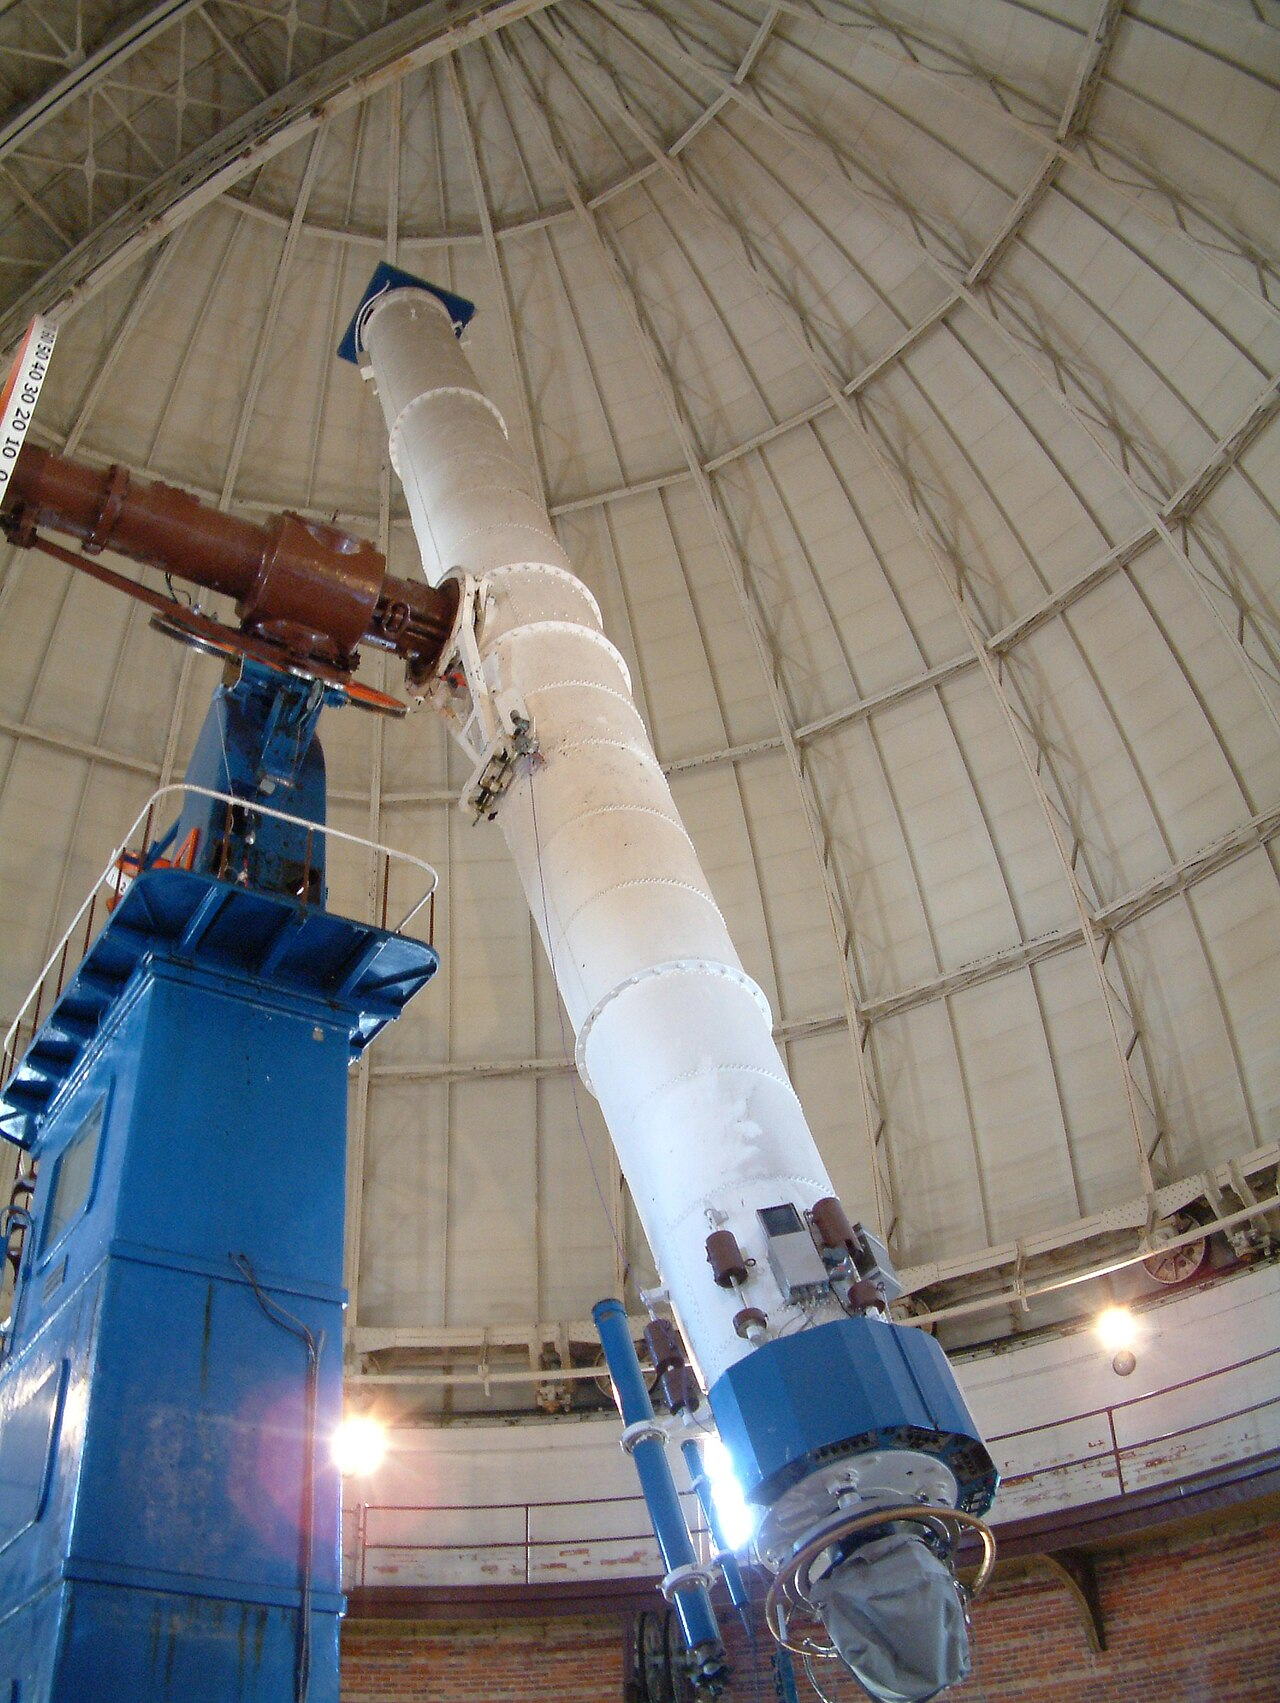
\includegraphics[width=0.42\linewidth]{images/book3/yerkes-refractor.jpg}

{\small 叶凯士天文台的 40 英寸折射望远镜（1897 年），至今仍是有史以来最大的\omterm{def:b1:mirrors-thin-lenses:lens}{透镜}望远镜：\omterm{def:b1:optical-instruments:microscope}{物镜}直径一米，镜筒长十九米。超过这一尺寸，\omterm{def:b1:mirrors-thin-lenses:lens}{透镜}就会在自身重量下下垂，天文学于是转向反射镜。}
\end{omfigure}

\begin{omfigure}
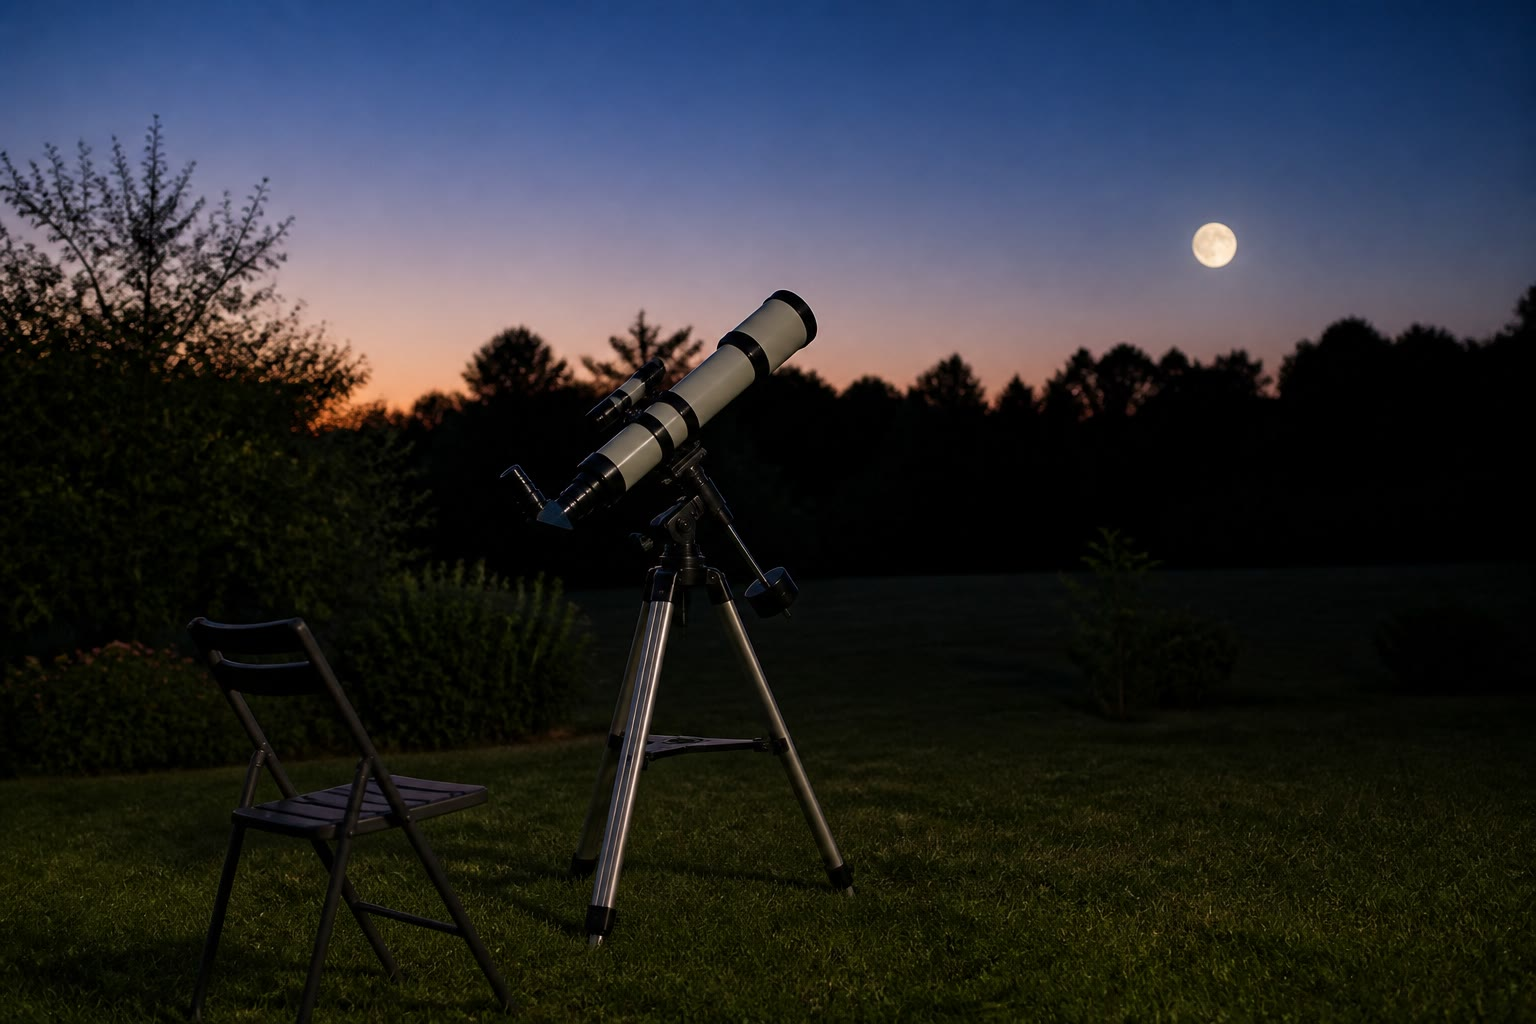
\includegraphics[width=0.58\linewidth]{images/book3/ai/b3-04-telescope-dusk.jpg}

{\small 黄昏时分的一台小型折射望远镜：\omterm{def:b1:optical-instruments:microscope}{物镜}\omterm{def:b1:mirrors-thin-lenses:lens}{焦距}长，\omterm{def:b1:optical-instruments:microscope}{目镜}\omterm{def:b1:mirrors-thin-lenses:lens}{焦距}短——即本章所讨论的无焦望远镜，对准的是其周末问题中的月球。}
\end{omfigure}

\section{眼睛}

\begin{definition}[简化眼]\label{def:b1:optical-instruments:eye}
\index{眼睛}\index{简化眼}\index{视网膜}\index{调节}
\emph{简化眼}把角膜与晶状体等效为一片\omterm{def:b1:mirrors-thin-lenses:lens}{焦距}
\emph{可变}的薄\omterm{def:b1:mirrors-thin-lenses:lens}{凸透镜}，并把\emph{视网膜}看作
位于其后、距离固定为 $d \approx \qty{17}{mm}$ 的屏幕。
肌肉改变晶状体的曲率，使所看物体的像
始终成在视网膜上，这就是\emph{调节}。位于\omterm{def:b1:mirrors-thin-lenses:lens}{透镜}前方的虹膜
是一个可变光阑，其孔径在 \qty{2}{} 至
\qty{8}{mm} 之间，即\emph{瞳孔}。
\end{definition}

\begin{definition}[远点、近点]\label{def:b1:optical-instruments:punctum}
\index{远点}\index{近点}\index{调节幅度}
\emph{远点}（punctum remotum）是指不经\omterm{def:b1:optical-instruments:eye}{调节}即可清晰看到的
物点；\emph{近点}（punctum proximum）是指在最大\omterm{def:b1:optical-instruments:eye}{调节}下
能清晰看到的最近的点。对正常眼而言，远点位于无穷远，
近点位于 $d_m \approx \qty{25}{cm}$ 处，
这一距离即常规的\emph{明视距离}。
两者所需\omterm{def:b1:mirrors-thin-lenses:lens}{光焦度}之差即为\emph{\omterm{def:b1:optical-instruments:eye}{调节}幅度}，
对青年人约为 \qty{4}{\delta}，
并随年龄增长而下降。
\end{definition}

\begin{example}[眼睛的光焦度]\label{ex:b1:optical-instruments:vergence}
远处物体：像位于 $d = \qty{17}{mm}$ 处，故 $f' = \qty{17}{mm}$，
$V = 1/0.017 = \qty{59}{\delta}$。物体位于 \qty{25}{cm} 处时：
$V = 1/0.017 + 1/0.25 = 59 + 4 = \qty{63}{\delta}$。在六十屈光度中，
\omterm{def:b1:optical-instruments:eye}{调节}只占四屈光度：晶状体所贡献的仅为角膜工作量的百分之几，
但这百分之几对阅读而言却至关重要。
\end{example}

\begin{proposition}[缺陷与矫正]\label{prop:b1:optical-instruments:defects}
\index{近视}\index{远视}\index{老花眼}
\emph{\omterm{prop:b1:optical-instruments:defects}{近视}}眼的会聚能力过强：其\omterm{def:b1:optical-instruments:punctum}{远点}位于有限距离 $D_r$ 处；
\omterm{def:b1:mirrors-thin-lenses:lens}{焦距}为 $f' = -D_r$ 的\omterm{def:b1:mirrors-thin-lenses:lens}{凹透镜}（紧贴眼前佩戴）
将无穷远处的物成像于\omterm{def:b1:optical-instruments:punctum}{远点}，从而恢复远距视力。
\emph{\omterm{prop:b1:optical-instruments:defects}{远视}}眼的会聚能力不足：其\omterm{def:b1:optical-instruments:punctum}{远点}为虚点（位于眼后），
\omterm{def:b1:optical-instruments:punctum}{近点}又过远；\omterm{def:b1:mirrors-thin-lenses:lens}{凸透镜}可以矫正之。
\emph{\omterm{prop:b1:optical-instruments:defects}{老花眼}}是指随年龄增长而丧失\omterm{def:b1:optical-instruments:eye}{调节}能力，
\omterm{def:b1:optical-instruments:punctum}{近点}后移，阅读需要\omterm{def:b1:mirrors-thin-lenses:lens}{凸透镜}，
而与\omterm{def:b1:optical-instruments:punctum}{远点}状况无关。
\end{proposition}

\begin{proof}
紧贴眼前的\omterm{def:b1:mirrors-thin-lenses:lens}{透镜}与\omterm{def:b1:optical-instruments:eye}{眼睛}构成一个系统，其物须是
\omterm{def:b1:optical-instruments:eye}{眼睛}所能看见的：\omterm{def:b1:mirrors-thin-lenses:lens}{透镜}必须把无穷远处的物体变成位于\omterm{def:b1:optical-instruments:punctum}{远点}的
\omterm{def:b1:mirrors-thin-lenses:image}{虚像}，其中 $\overline{OA'} = -D_r$，
$\overline{OA} = -\infty$，故 $f' = \overline{OA'} = -D_r$。其余情形的论证与此相同，
只需将相应的点代入即可。
\end{proof}

\begin{omfigure}
\begin{tikzpicture}[font=\small, x=1cm, y=1cm]
  % eye schematic: lens at x=0, retina at x=2.4 (scaled), object far (parallel rays) and near
  \draw[omDef!30, fill=omDef!8] (1.25,0) ellipse (1.45 and 1.15);
  \draw[very thick, omDef, Stealth-Stealth] (0,-0.8) -- (0,0.8);
  \draw[very thick, omThm] (2.6,-0.55) arc (-25:25:1.3);
  \node[omThm, right] at (2.75,0.9) {视网膜};
  \node[omDef, above] at (0,0.85) {透镜};
  % far object: parallel rays -> focus on retina at axis
  \draw[omProp, -Stealth] (-3.2,0.5) -- (0,0.5); \draw[omProp] (0,0.5) -- (2.58,0);
  \draw[omProp, -Stealth] (-3.2,-0.5) -- (0,-0.5); \draw[omProp] (0,-0.5) -- (2.58,0);
  \draw[-Stealth] (-3.4,0) -- (3.3,0);
  \node[omProp, left] at (-3.2,0.5) {远处物体};
  \draw[Stealth-Stealth] (0,-1.35) -- (2.58,-1.35) node[midway, below] {$d \approx \qty{17}{mm}$};
  % near object at x=-2.4 height 0.6 : with accommodation image at retina: drawn as converging rays from B through O
  \begin{scope}[xshift=7.6cm]
  \draw[omDef!30, fill=omDef!8] (1.25,0) ellipse (1.45 and 1.15);
  \draw[very thick, omDef, Stealth-Stealth] (0,-0.8) -- (0,0.8);
  \draw[very thick, omThm] (2.6,-0.55) arc (-25:25:1.3);
  \draw[-Stealth] (-3.4,0) -- (3.3,0);
  \draw[very thick, omThm, -Stealth] (-2.6,0) -- (-2.6,0.6); \node[above] at (-2.6,0.6) {$B$};
  \draw[omProp] (-2.6,0.6) -- (0,0.6) -- (2.58,-0.6);
  \draw[omProp] (-2.6,0.6) -- (0,0.0) -- (2.58,-0.6);
  \draw[omProp] (-2.6,0.6) -- (0,-0.6) -- (2.58,-0.6);
  \node[omThm, below right] at (2.55,-0.6) {$B'$};
  \node[below] at (-0.4,-1.3) {调节时：$f'$ 缩短};
  \end{scope}
\end{tikzpicture}

{\small \omterm{def:b1:optical-instruments:eye}{简化眼}：一片\omterm{def:b1:mirrors-thin-lenses:lens}{焦距}可变的\omterm{def:b1:mirrors-thin-lenses:lens}{薄透镜}，其后方
\qty{17}{mm} 处为\omterm{def:b1:optical-instruments:eye}{视网膜}。放松时，它聚焦远处物体；
\omterm{def:b1:optical-instruments:eye}{调节}时，它缩短 $f'$，使近处物体的像落在\omterm{def:b1:optical-instruments:eye}{视网膜}上。
成像是倒立的——大脑会将其翻转过来。}
\end{omfigure}

\begin{definition}[视角与角分辨率]\label{def:b1:optical-instruments:angular}
\index{视角}\index{角分辨率}
高为 $h$、距离为 $D$ 的物体的\emph{视角}为
$\theta \approx h/D$（小角度）。人眼能分辨两点，
当且仅当其角间距超过自身的\emph{角分辨率}，
约为 $\epsilon \approx \qty{3e-4}{rad}$（即一角分）：
视锥细胞的间距与瞳孔处的衍射共同决定了这一极限。
\end{definition}

\begin{remark}[仪器的用途]\label{rem:b1:optical-instruments:purpose}
将物体置于\omterm{def:b1:optical-instruments:punctum}{近点}时，\qty{1}{mm} 的细节所对\omterm{def:b1:optical-instruments:angular}{视角}为 $1/250 =
\qty{4e-3}{rad}$：是分辨极限的十三倍；\qty{0.05}{mm}
的细节所对\omterm{def:b1:optical-instruments:angular}{视角}为 $\qty{2e-4}{rad}$，不可见。用于观察近处物体的仪器
（\omterm{def:b1:optical-instruments:G}{放大镜}、\omterm{def:b1:optical-instruments:microscope}{显微镜}）使\omterm{def:b1:optical-instruments:angular}{视角}增大的程度，超过将物体移近所能做到的；
用于远处物体的仪器（望远镜）则增大了无法靠近之物的\omterm{def:b1:optical-instruments:angular}{视角}；
\omterm{def:b1:optical-instruments:camera}{照相机}以一种可对光积分的传感器取代\omterm{def:b1:optical-instruments:eye}{视网膜}，
该传感器可累积数秒的光，
并可事后放大。
\end{remark}

\section{放大镜}

\begin{definition}[角放大率]\label{def:b1:optical-instruments:G}
\index{角放大率}\index{放大镜}\index{标称放大率}
对于供人眼使用的仪器，其\emph{角放大率}为
$G = \theta'/\theta$，其中 $\theta'$ 为经仪器所见像的\omterm{def:b1:optical-instruments:angular}{视角}，
$\theta$ 为肉眼所见物体的\omterm{def:b1:optical-instruments:angular}{视角}，
即对近处物体取\omterm{def:b1:optical-instruments:punctum}{近点} $d_m = \qty{25}{cm}$ 处，
对远处物体则无需移动。
\end{definition}

\begin{proposition}[放大镜]\label{prop:b1:optical-instruments:loupe}
\omterm{def:b1:mirrors-thin-lenses:lens}{焦距}为 $f' < d_m$ 的\omterm{def:b1:mirrors-thin-lenses:lens}{凸透镜}，物体位于其
物方焦平面上时，所成像位于无穷远，无需\omterm{def:b1:optical-instruments:eye}{调节}即可观察，
放大率为
\[
G = \frac{d_m}{f'} = d_m V .
\]
\end{proposition}

\begin{proof}
物 $AB$ 高为 $h$，位于焦平面上：自 $B$ 发出的光线
平行射出，角度与过 $O$ 点的光线相同，$\theta' = h/f'$。不借助仪器时
肉眼处于\omterm{def:b1:optical-instruments:punctum}{近点}：$\theta = h/d_m$。于是比值为 $d_m/f'$。
\end{proof}

\begin{example}[钟表匠的放大镜]\label{ex:b1:optical-instruments:loupe}
$f' = \qty{25}{mm}$：$G = 250/25 = 10$，标称为“$10\times$”。此时
\qty{0.05}{mm} 的细节所对\omterm{def:b1:optical-instruments:angular}{视角}为 $\qty{2e-3}{rad}$，
若要进一步提高 $G$，则需\omterm{def:b1:mirrors-thin-lenses:lens}{焦距} $f'$ 仅为几毫米的
微型\omterm{def:b1:mirrors-thin-lenses:lens}{透镜}紧贴于眼前——这是单\omterm{def:b1:mirrors-thin-lenses:lens}{透镜}的极限，
也正是\omterm{def:b1:optical-instruments:microscope}{显微镜}存在的原因。
\end{example}

\section{显微镜}

\begin{definition}[复式显微镜]\label{def:b1:optical-instruments:microscope}
\index{显微镜}\index{物镜}\index{目镜}\index{光学筒长}
\emph{显微镜}是由\omterm{def:b1:mirrors-thin-lenses:lens}{焦距}较短的\emph{物镜} $L_1$，
\omterm{def:b1:mirrors-thin-lenses:lens}{焦距}为 $f_1'$，对近处物体形成实的、放大的中间像，
该中间像位于\emph{目镜} $L_2$ 的物方焦平面上（\omterm{def:b1:mirrors-thin-lenses:lens}{焦距}为
$f_2'$），起\omterm{def:b1:optical-instruments:G}{放大镜}的作用。物镜像方焦点与目镜物方焦点间的距离 $\Delta =
\overline{F_1'F_2}$，
即\emph{光学筒长}，经典仪器上标准化取为
\qty{160}{mm}。
\end{definition}

\begin{proposition}[显微镜的放大率]\label{prop:b1:optical-instruments:microscope}
最终像位于无穷远时，
\[
\gamma_1 = -\frac{\Delta}{f_1'}, \qquad G_2 = \frac{d_m}{f_2'},
\qquad G = \abs{\gamma_1}\,G_2 = \frac{\Delta\,d_m}{f_1' f_2'} .
\]
\end{proposition}

\begin{proof}
中间像 $A_1B_1$ 位于\omterm{def:b1:optical-instruments:microscope}{目镜}的物方焦平面上，
即在 $\overline{F_1'A_1} = \Delta$ 处；由牛顿公式可得
$\gamma_1 = -\overline{F_1'A_1}/f_1' = -\Delta/f_1'$。\omterm{def:b1:optical-instruments:microscope}{目镜}随后将
$A_1B_1$（高为 $\abs{\gamma_1} h$）送至无穷远，\omterm{def:b1:optical-instruments:angular}{视角}为
$\theta' = \abs{\gamma_1} h/f_2'$，与肉眼观察时的
$\theta = h/d_m$ 相比。
\end{proof}

\begin{omfigure}
\begin{tikzpicture}[font=\small, x=1cm, y=1cm]
  % objective L1 at 0, f1'=0.8 ; object at OA=-1.12 -> OA'=2.8, gamma=-2.5 ; eyepiece L2 at 3.8 (f2'=1), F2 = 2.8
  \draw[-Stealth] (-1.9,0) -- (6.7,0);
  \draw[very thick, omDef, Stealth-Stealth] (0,-1.3) -- (0,1.3); \node[omDef, above] at (0,1.35) {物镜 $L_1$};
  \draw[very thick, omDef, Stealth-Stealth] (3.8,-1.7) -- (3.8,1.7); \node[omDef, above] at (3.8,1.75) {目镜 $L_2$};
  \foreach \x/\n in {-0.8/F_1, 0.8/F_1', 4.8/F_2'} {\fill (\x,0) circle (1.2pt); \node[below] at (\x,-0.05) {$\n$};}
  \fill (2.8,0) circle (1.2pt); \node[above right] at (2.8,0.02) {$F_2$};
  \draw[very thick, omThm, -Stealth] (-1.12,0) -- (-1.12,0.3); \node[above left] at (-1.12,0.3) {$B$};
  \draw[very thick, omThm, -Stealth] (2.8,0) -- (2.8,-0.75); \node[below left] at (2.8,-0.75) {$B_1$};
  \draw[omProp] (-1.12,0.3) -- (0,0.3) -- (2.8,-0.75);
  \draw[omProp] (-1.12,0.3) -- (0,0) -- (2.8,-0.75);
  \draw[omExo] (2.8,-0.75) -- (3.8,-0.75) -- (6.2,1.05);
  \draw[omExo] (2.8,-0.75) -- (3.8,0) -- (6.2,1.8);
  \draw[omExo] (2.8,-0.75) -- (3.8,-1.5) -- (6.2,0.3);
  \draw[Stealth-Stealth] (0.8,0.5) -- (2.8,0.5) node[midway, above] {$\Delta$};
  \node[omExo, right] at (6.25,0.75) {射向人眼};
\end{tikzpicture}

{\small \omterm{def:b1:optical-instruments:microscope}{显微镜}：\omterm{def:b1:optical-instruments:microscope}{物镜}形成一个实的、放大的、
倒立的中间像 $A_1B_1$，位于\omterm{def:b1:optical-instruments:microscope}{目镜}的物方焦平面上；
\omterm{def:b1:optical-instruments:microscope}{目镜}将其送至无穷远，放松状态下的人眼
以较大的\omterm{def:b1:optical-instruments:angular}{视角}观察它。}
\end{omfigure}

\begin{example}[学生用显微镜]\label{ex:b1:optical-instruments:micronum}
\omterm{def:b1:optical-instruments:microscope}{物镜} $f_1' = \qty{4.0}{mm}$，\omterm{def:b1:optical-instruments:microscope}{目镜} $f_2' = \qty{25}{mm}$，
$\Delta = \qty{160}{mm}$：$\gamma_1 = -40$，$G_2 = 10$，$G = 400$。物体
位于 $\overline{F_1A} = -f_1'^2/\Delta = -16/160 =
\qty{-0.10}{mm}$ 处，即距 $F_1$ 为该值，距\omterm{def:b1:optical-instruments:microscope}{物镜} \qty{4.1}{mm}。调焦
意味着整体移动镜筒，移动量仅为毫米的几分之一。
\end{example}

\begin{remark}[分辨极限]\label{rem:b1:optical-instruments:abbe}
\index{分辨本领}
放大倍数若不受限制则毫无用处：光是一种波，\omterm{def:b1:optical-instruments:microscope}{物镜}接收
半角为 $u$ 的光线（介质折射率为 $n$）时，无法分辨
间距小于约 $\lambda/(2n\sin u)$ 的两点
——此式由本科二年级分册的波动理论推出。
取 $n\sin u \approx 1.4$（油浸\omterm{def:b1:optical-instruments:microscope}{物镜}），$\lambda =
\qty{0.5}{\micro m}$，极限约为 \qty{0.2}{\micro m}。要使
这一细节为人眼所见（$\epsilon = \qty{3e-4}{rad}$
在 \qty{25}{cm} 处即 \qty{75}{\micro m}），放大约 $400$
即可；超过 $1000$ 倍后，像只是变大而不更丰富：
\emph{空放大}。
\end{remark}

\section{天文望远镜}

\begin{proposition}[折射式望远镜]\label{prop:b1:optical-instruments:telescope}
\index{望远镜}\index{出瞳}
\omterm{def:b1:optical-instruments:microscope}{物镜} $L_1$ 与\omterm{def:b1:optical-instruments:microscope}{目镜} $L_2$ 满足 $F_1' = F_2$，组成一个
\omterm{prop:b1:mirrors-thin-lenses:doublet}{无焦系统}：来自恒星（无穷远）的光经其成像于无穷远，放松状态下的人眼
可直接观察之，且
\[
G = -\frac{f_1'}{f_2'} .
\]
\omterm{def:b1:optical-instruments:microscope}{物镜}边缘经\omterm{def:b1:optical-instruments:microscope}{目镜}所成的像是
\emph{\omterm{prop:b1:optical-instruments:telescope}{出瞳}}：直径为 $D/\abs G$ 的亮圆盘，位于
\omterm{def:b1:optical-instruments:microscope}{目镜}后方 $\overline{O_2P'} = f_2'(f_1' + f_2')/f_1'$ 处，
人眼瞳孔须置于此处，方能接收全部光线。
\end{proposition}

\begin{proof}
$G$ 由\cref{prop:b1:mirrors-thin-lenses:doublet}推出。
从 $L_2$ 看，\omterm{def:b1:optical-instruments:microscope}{物镜}是位于 $\overline{O_2O_1} = -(f_1'
+ f_2')$ 处的物体；由笛卡儿公式得 $1/\overline{O_2P'} = 1/f_2' - 1/(f_1' + f_2')
= f_1'/[f_2'(f_1' + f_2')]$，放大率为 $\overline{O_2P'}/
\overline{O_2O_1} = -f_2'/f_1' = 1/G$，即直径 $D$ 缩放为 $D/\abs G$。
进入\omterm{def:b1:optical-instruments:microscope}{物镜}的每一条光线都经\omterm{prop:b1:optical-instruments:telescope}{出瞳}射出，
因为\omterm{def:b1:optical-instruments:microscope}{物镜}上每一点都在此成像。
\end{proof}

\begin{omfigure}
\begin{tikzpicture}[font=\small, x=1cm, y=1cm]
  % objective f1'=4 at x=0 ; eyepiece f2'=1 at x=5 ; parallel beam at angle alpha -> focus at height -4*alpha; take alpha such that height 0.5: rays entering at heights 1, 0, -1 with slope -0.125
  \draw[-Stealth] (-2.2,0) -- (7.8,0);
  \draw[very thick, omDef, Stealth-Stealth] (0,-1.4) -- (0,1.4); \node[omDef, above] at (0,1.45) {物镜 $L_1$，$D$};
  \draw[very thick, omDef, Stealth-Stealth] (5,-0.8) -- (5,0.8); \node[omDef, above] at (5,0.85) {目镜 $L_2$};
  \fill (4,0) circle (1.2pt); \node[above] at (4,0.08) {$F_1' = F_2$};
  % beam from a star at angle: parallel rays slope -0.125 entering at y=1.25,0.25,-0.75 then reaching lens; then to focus (4,-0.5)
  \foreach \y in {1.2,0.0,-1.2} {
    \draw[omProp] (-2.0,\y+0.25) -- (0,\y);
    \draw[omProp] (0,\y) -- (4,-0.5);
    % after eyepiece: parallel, slope = +0.5/1 -> direction from (5, y2) with slope 0.5; y2 = -0.5 + (4,-0.5)->(5,?) line through focus continuing: ray from (0,\y) to (4,-0.5) extended to x=5: y = -0.5 + (-0.5-\y)/4
    \draw[omExo] (4,-0.5) -- (5,{-0.5+(-0.5-\y)/4}) -- (7.6,{-0.5+(-0.5-\y)/4+1.3});
  }
  % exit pupil: image of objective rim: O2P' = 1*5/4 = 1.25 beyond L2 ; diameter D/G = 2.4/4 = 0.6
  \draw[very thick, omThm] (6.25,-0.3) -- (6.25,0.3); \node[omThm, below] at (6.4,-0.8) {出瞳 $D/\abs{G}$};
  \node[omProp, left] at (-2.0,1.45) {来自恒星};
\end{tikzpicture}

{\small 天文望远镜：来自恒星的平行光束
经\omterm{def:b1:optical-instruments:microscope}{物镜}在公共焦平面上聚焦，再经\omterm{def:b1:optical-instruments:microscope}{目镜}射向无穷远，
角度放大为 $\abs G$ 倍。直径为 $D$ 的\omterm{def:b1:optical-instruments:microscope}{物镜}所收集的全部光线，
都经过直径为 $D/\abs G$ 的
\omterm{prop:b1:optical-instruments:telescope}{出瞳}。}
\end{omfigure}

\begin{proposition}[望远镜的增益]\label{prop:b1:optical-instruments:gains}
\index{集光本领}\index{瑞利判据}
与裸眼（瞳孔直径 $d_p$）相比：
\begin{itemize}
  \item \emph{\omterm{def:b1:optical-instruments:angular}{视角}}：放大 $\abs G$ 倍；
  \item \emph{所集光能}（对点光源）：放大为
        $(D/d_p)^2$ 倍，前提是\omterm{prop:b1:optical-instruments:telescope}{出瞳}不大于
        人眼瞳孔，即 $\abs G \geq D/d_p$；
  \item \emph{\omterm{def:b1:optical-instruments:angular}{角分辨率}}：\omterm{def:b1:optical-instruments:microscope}{物镜}处的衍射将其限制为
        $\theta_{\min} \approx 1.22\,\lambda/D$（瑞利判据），
        远小于人眼的 $\epsilon$；使这一极限可见的放大率
        为 $G_r = \epsilon/\theta_{\min}$，
        更大的放大率只会放大模糊。
\end{itemize}
\end{proposition}
\admitted

\begin{example}[业余爱好者的 150 毫米折射望远镜]\label{ex:b1:optical-instruments:telnum}
$D = \qty{150}{mm}$，$f_1' = \qty{1200}{mm}$，\omterm{def:b1:optical-instruments:microscope}{目镜} \qty{25}{mm}：
$G = -48$；\omterm{prop:b1:optical-instruments:telescope}{出瞳} \qty{3.1}{mm}；集光增益为 $(150/7)^2 \approx
460$（与暗适应瞳孔 \qty{7}{mm} 相比）；分辨率 $1.22 \times
\qty{550}{nm}/\qty{0.15}{m} = \qty{4.5e-6}{rad} = 0.9''$，故
月球上宽 \qty{1.7}{km} 的环形山可以分辨；$G_r = 3\times10^{-4}/4.5\times
10^{-6} \approx 67$——用 \qty{6}{mm} \omterm{def:b1:optical-instruments:microscope}{目镜}（$G = 200$）看不到
更多细节，只会得到更暗、更大的圆盘。
周末问题要求设计此仪器。
\end{example}

\begin{remark}[反射式望远镜、双筒望远镜与单筒望远镜]\label{rem:b1:optical-instruments:variants}
\omterm{def:b1:mirrors-thin-lenses:lens}{焦距}为 $f_1'$ 的\omterm{def:b1:mirrors-thin-lenses:mirror}{凹面镜}取代\omterm{def:b1:optical-instruments:microscope}{物镜}\omterm{def:b1:mirrors-thin-lenses:lens}{透镜}，
构成\emph{反射式}望远镜（无色散，且反射镜
可以做到数米宽，并可从背面支撑）：上述内容均成立，
只需将 $f_1'$ 理解为反射镜的\omterm{def:b1:mirrors-thin-lenses:lens}{焦距}。成像是倒立的——
观测恒星时无妨；用于地面观测时，双筒望远镜中插入一对
\omterm{thm:b1:rays-reflection-refraction:tir}{全反射}棱镜使像正立；伽利略望远镜采用
\omterm{def:b1:mirrors-thin-lenses:lens}{凹透镜}作\omterm{def:b1:optical-instruments:microscope}{目镜}（$f_2' < 0$，$G > 0$），较短，但
视场狭窄。
\end{remark}

\section{照相机}

\begin{definition}[照相机；光圈数]\label{def:b1:optical-instruments:camera}
\index{照相机}\index{光圈数}\index{景深}
\emph{照相机}是\omterm{def:b1:mirrors-thin-lenses:lens}{焦距}为 $f'$ 的会聚\omterm{def:b1:mirrors-thin-lenses:lens}{透镜}，
在感光元件上成\omterm{def:b1:mirrors-thin-lenses:image}{实像}，对远处物体，$\overline{OA'} \approx f'$；
调焦时移动\omterm{def:b1:mirrors-thin-lenses:lens}{透镜}。直径为 $D$ 的光阑限制光束；
\emph{光圈数}为 $N = f'/D$（写作 $f/N$）。\emph{视场角}
为 $2\arctan(\ell/2f')$（感光元件宽度为 $\ell$）。
\end{definition}

\begin{proposition}[曝光与景深]\label{prop:b1:optical-instruments:dof}
\index{超焦距}
感光元件上的辐照度与 $1/N^2$ 成正比，
因此对给定的像亮度，曝光时间与 $N^2$ 成正比。
与对\omterm{def:b1:mirrors-thin-lenses:lens}{焦距}离不同的点会成一个弥散圆；
要求其直径不超过允许值 $c$，则\omterm{def:b1:mirrors-thin-lenses:lens}{透镜}对焦于\emph{\omterm{prop:b1:optical-instruments:dof}{超焦
距}}，记为
\[
H = \frac{f'^2}{N c}
\]
此时从 $H/2$ 到无穷远的所有物体都能清晰成像。
\end{proposition}

\begin{proof}
辐照度 $=$ 功率/面积 $\propto D^2/f'^2 = 1/N^2$（给定物体的像
大小由 $f'$ 决定，收集的功率随 $D^2$ 增长）。
对焦于距离 $p$ 处，像位于 $q \approx f'$；
无穷远处的点聚焦于 $f'$，即在感光元件前 $q - f'$ 处；
其光锥在\omterm{def:b1:mirrors-thin-lenses:lens}{透镜}处底面直径为 $D$，在感光元件上的直径为 $D(q - f')/q$
（相似三角形）。在近轴近似下，$1/q = 1/f' - 1/p$，
因此 $q - f' \approx f'^2/p$（$p \gg f'$），于是弥散圆为
$Df'/p = f'^2/(Np)$，令其等于 $c$ 得 $p = H$。
同一几何关系用于近侧，得到极限 $H/2$。
\end{proof}

\begin{omfigure}
\begin{tikzpicture}[font=\small, x=1cm, y=1cm]
  \draw[-Stealth] (-5.5,0) -- (2.6,0);
  \draw[very thick, omDef, Stealth-Stealth] (0,-1.2) -- (0,1.2); \node[omDef, above] at (0,1.25) {透镜，孔径 $D$};
  \draw[very thick] (1.8,-1.3) -- (1.8,1.3); \node[right] at (1.8,1.1) {感光元件};
  % focused point at x=-4 (p) images at q=1.8 ; far point at infinity images at f'=1.5
  \fill[omThm] (-4,0) circle (1.5pt); \node[below left, omThm] at (-4,-0.05) {对焦点};
  \draw[omThm] (-4,0) -- (0,1.0) -- (1.8,0); \draw[omThm] (-4,0) -- (0,-1.0) -- (1.8,0);
  % far point: parallel rays focus at 1.5, then diverge to sensor making blur
  \draw[omProp] (-5.3,1.0) -- (0,1.0) -- (1.5,0) -- (1.8,-0.2);
  \draw[omProp] (-5.3,-1.0) -- (0,-1.0) -- (1.5,0) -- (1.8,0.2);
  \draw[very thick, omProp] (1.82,-0.2) -- (1.82,0.2); \node[omProp, right] at (1.85,-0.35) {弥散圆 $c$};
  \node[omProp, left] at (-5.3,1.0) {远点};
  \fill (1.5,0) circle (1.2pt); \node[below] at (1.5,-0.05) {$F'$};
\end{tikzpicture}

{\small \omterm{def:b1:optical-instruments:camera}{景深}：\omterm{def:b1:mirrors-thin-lenses:lens}{透镜}对焦于距离为 $p$ 的点
（像位于感光元件上）；无穷远处的点聚焦于感光元件前的 $F'$，
留下直径为 $c = Df'/p$ 的弥散圆——光圈越小，
即 $N$ 越大时弥散圆越小，
因此清晰度与曝光时间需要权衡。}
\end{omfigure}

\begin{example}[全画幅与手机]\label{ex:b1:optical-instruments:cameras}
一个 \qty{50}{mm} 的镜头配 \qty{36}{mm} 宽的感光元件：视场角
$2\arctan(18/50) = 40^\circ$；在 $f/8$、$c = \qty{0.03}{mm}$ 时，
$H = 2500/(8 \times 0.03) = \qty{10}{m}$：对焦于 \qty{10}{m}，
超过 \qty{5}{m} 的物体都清晰。手机镜头 $f' = \qty{4.3}{mm}$，
在 $f/1.8$ 下配 \qty{6}{mm} 宽的感光元件，$c = \qty{5}{\micro m}$，
视场角相同（宽 \qty{70}{\degree}），$H = 18.5/(1.8 \times 0.005) =
\qty{2.1}{m}$——几乎所有物体同时清晰成像，
这就是手机用软件模拟背景虚化的原因。
\end{example}

\begin{omfigure}
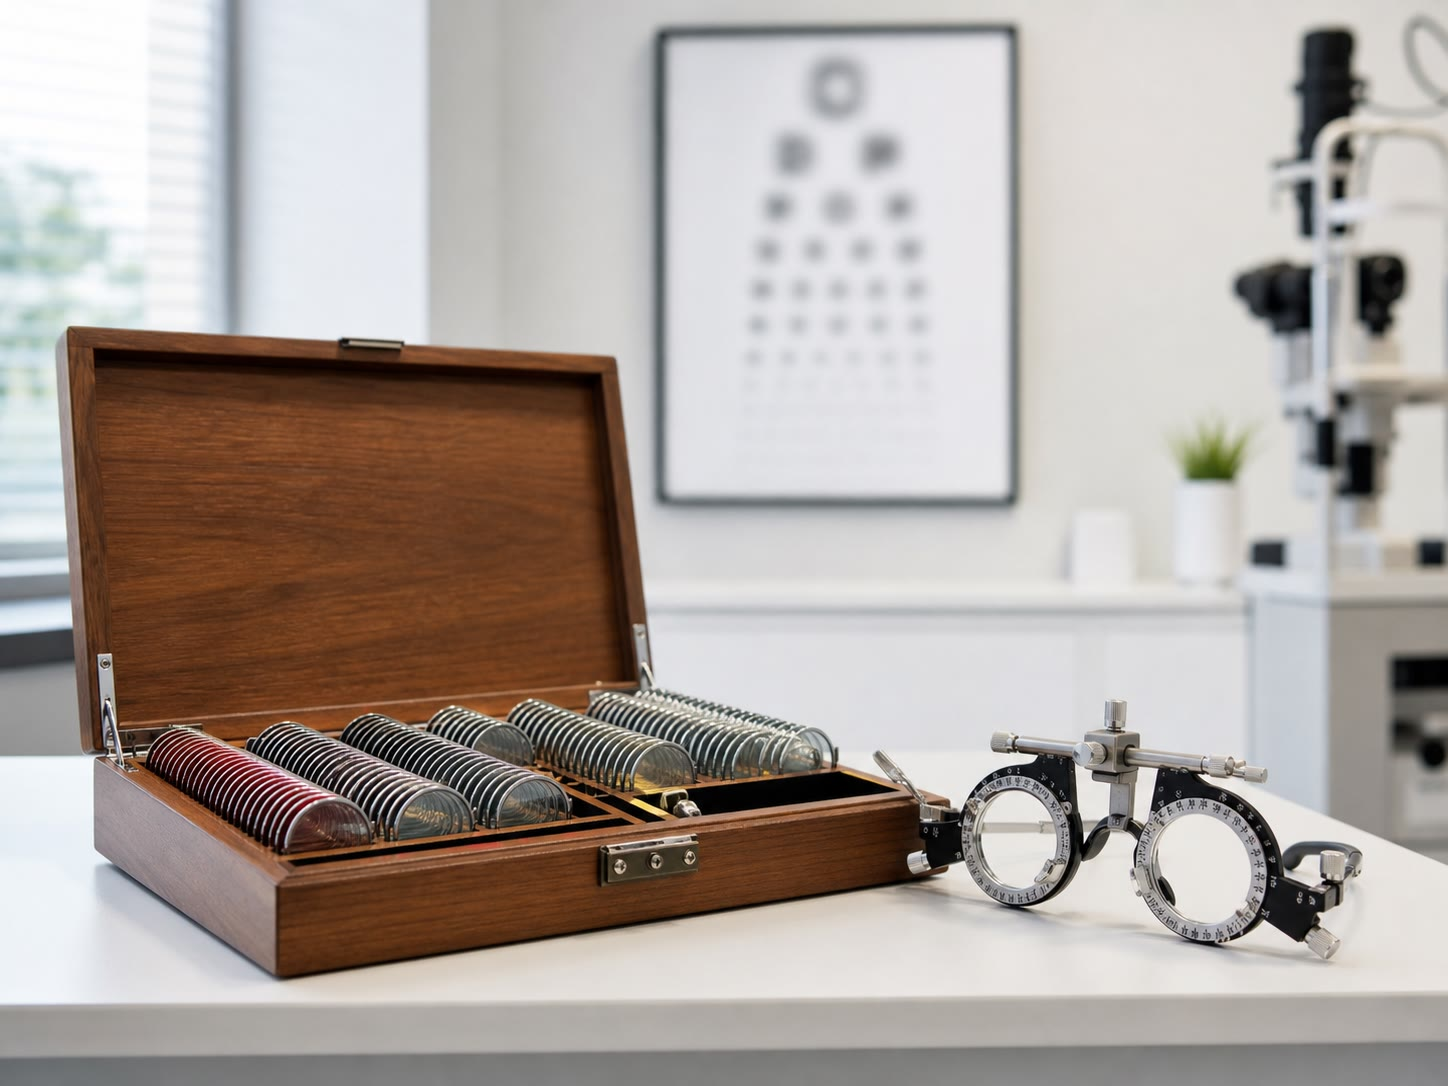
\includegraphics[width=0.50\linewidth]{images/book3/ai/b3-04-eye-chart-trial-frame.jpg}

{\small 验光师的试镜片与试镜架：在眼前放置合适\omterm{def:b1:mirrors-thin-lenses:lens}{光焦度}的\omterm{def:b1:mirrors-thin-lenses:lens}{凸透镜}或\omterm{def:b1:mirrors-thin-lenses:lens}{凹透镜}，可将其\omterm{def:b1:optical-instruments:punctum}{远点}移回无穷远。}
\end{omfigure}

\section{练习}

\begin{exercise}[$\star$]\label{exo:b1:optical-instruments:1}
\omterm{def:b1:optical-instruments:eye}{视网膜}位于\omterm{def:b1:mirrors-thin-lenses:lens}{透镜}后 \qty{17}{mm} 处，
求正常眼观察无穷远及 \qty{25}{cm} 处物体时的\omterm{def:b1:mirrors-thin-lenses:lens}{光焦度}，
并推算\omterm{def:b1:optical-instruments:punctum}{调节幅度}。这些对应的\omterm{def:b1:mirrors-thin-lenses:lens}{焦距}各为多少？
\end{exercise}

\begin{exercise}[$\star$]\label{exo:b1:optical-instruments:2}
\omterm{prop:b1:optical-instruments:defects}{近视}眼的\omterm{def:b1:optical-instruments:punctum}{远点}位于 \qty{40}{cm} 处。应配什么\omterm{def:b1:mirrors-thin-lenses:lens}{透镜}加以矫正
（求\omterm{def:b1:mirrors-thin-lenses:lens}{焦距}和\omterm{def:b1:mirrors-thin-lenses:lens}{光焦度}）？\omterm{prop:b1:optical-instruments:defects}{远视}眼的\omterm{def:b1:optical-instruments:punctum}{近点}为
\qty{1.0}{m}，应配什么\omterm{def:b1:mirrors-thin-lenses:lens}{透镜}才能使其看清 \qty{25}{cm} 处的文字？
\end{exercise}

\begin{exercise}[$\star$]\label{exo:b1:optical-instruments:3}
\omterm{def:b1:optical-instruments:G}{放大镜}的 $f' = \qty{4.0}{cm}$。求其\omterm{def:b1:optical-instruments:G}{角放大率}，
应将邮票置于何处，以及通过\omterm{def:b1:optical-instruments:G}{放大镜}看到的 \qty{2}{mm} 细节的\omterm{def:b1:optical-instruments:angular}{视角}，
并与明视距离 \qty{25}{cm} 处的裸眼相比较。
\end{exercise}

\begin{exercise}[$\star$]\label{exo:b1:optical-instruments:4}
折射望远镜的 $f_1' = \qty{900}{mm}$。求配 \qty{25}{mm}
与 \qty{9}{mm} \omterm{def:b1:optical-instruments:microscope}{目镜}时的 $G$，并求两种情形下的镜筒长度，
以及月球的视大小（$0.52^\circ$）。
\end{exercise}

\begin{exercise}[$\star\star$]\label{exo:b1:optical-instruments:5}
\omterm{def:b1:optical-instruments:microscope}{显微镜}：$f_1' = \qty{4.0}{mm}$，$f_2' = \qty{20}{mm}$，
$\Delta = \qty{160}{mm}$。求 $\gamma_1$、$G_2$、$G$ 以及
物体与\omterm{def:b1:optical-instruments:microscope}{物镜}之间的距离。镜筒应移动多少，
才能使物体深入 \qty{10}{\micro m} 处对焦？
\end{exercise}

\begin{exercise}[$\star\star$]\label{exo:b1:optical-instruments:6}
两盏前灯相距 \qty{1.5}{m}。在多远的距离上，
裸眼（$\epsilon = \qty{3e-4}{rad}$）才能分辨它们？一台望远镜
口径为 $D = \qty{100}{mm}$，求其衍射极限（$\lambda =
\qty{550}{nm}$），能分辨这两盏前灯的距离，以及
放大率 $G_r$ 超过多少后将不再显示新的细节。
\end{exercise}

\begin{exercise}[$\star\star$]\label{exo:b1:optical-instruments:7}
一个 \qty{50}{mm} 的镜头在 $f/2$ 时，其孔径直径是多少？某场景
在 $f/2$ 下以 $1/500$~\unit{s} 正确曝光，求在
$f/8$ 下的曝光时间，较小的光圈带来了什么好处？
\end{exercise}

\begin{exercise}[$\star\star$]\label{exo:b1:optical-instruments:8}
求 \qty{35}{mm} 镜头在 $f/11$ 时的\omterm{prop:b1:optical-instruments:dof}{超焦距}，取
$c = \qty{0.03}{mm}$，并求对焦于 $H$ 时的清晰距离范围。
街头摄影师为何要预先设定这一距离？
\end{exercise}

\begin{exercise}[$\star\star$]\label{exo:b1:optical-instruments:9}
双筒望远镜“$8\times30$”的 $G = 8$，$D = \qty{30}{mm}$。求
出射光瞳；若夜间瞳孔为 \qty{7}{mm}，光是否全部被利用？对于
“$7\times50$”呢？黄昏时哪一款更好，为何“$20\times30$”
是个糟糕的选择？
\end{exercise}

\begin{exercise}[$\star\star\star$]\label{exo:b1:optical-instruments:10}
\omterm{prop:b1:optical-instruments:defects}{近视}者的\omterm{def:b1:optical-instruments:punctum}{远点}距\omterm{def:b1:optical-instruments:eye}{眼睛} \qty{25}{cm}。求矫正用隐形眼镜的\omterm{def:b1:mirrors-thin-lenses:lens}{光焦度}，
再求框架眼镜的\omterm{def:b1:mirrors-thin-lenses:lens}{光焦度}，眼镜戴在眼前
\qty{15}{mm} 处。哪种矫正更强，
二者为何不同？
\end{exercise}

\begin{exercise}[$\star\star\star$]\label{exo:b1:optical-instruments:11}
伽利略望远镜：$f_1' = \qty{30}{cm}$，$f_2' = \qty{-10}{cm}$。求
使系统为\omterm{prop:b1:mirrors-thin-lenses:doublet}{无焦系统}时两\omterm{def:b1:mirrors-thin-lenses:lens}{透镜}的间距、$G$，以及
像的方向。确定出射光瞳的位置，并说明
视场为何较窄。
\end{exercise}

\begin{exercise}[$\star\star\star$]\label{exo:b1:optical-instruments:12}
一台 \qty{200}{mm} 的望远镜配 \qty{7}{mm} 的瞳孔，星光被增强了
多少倍？天文学家以星等标定亮度，
星等之差满足 $m_2 - m_1 = 2.5\log_{10}(F_1/F_2)$；\omterm{def:b1:optical-instruments:eye}{眼睛}能看到的星等
为 $6$ 的星，此望远镜的极限星等是多少？同一盏灯，
望远镜能看到的距离是肉眼的多少倍？
\end{exercise}

\begin{omfigure}
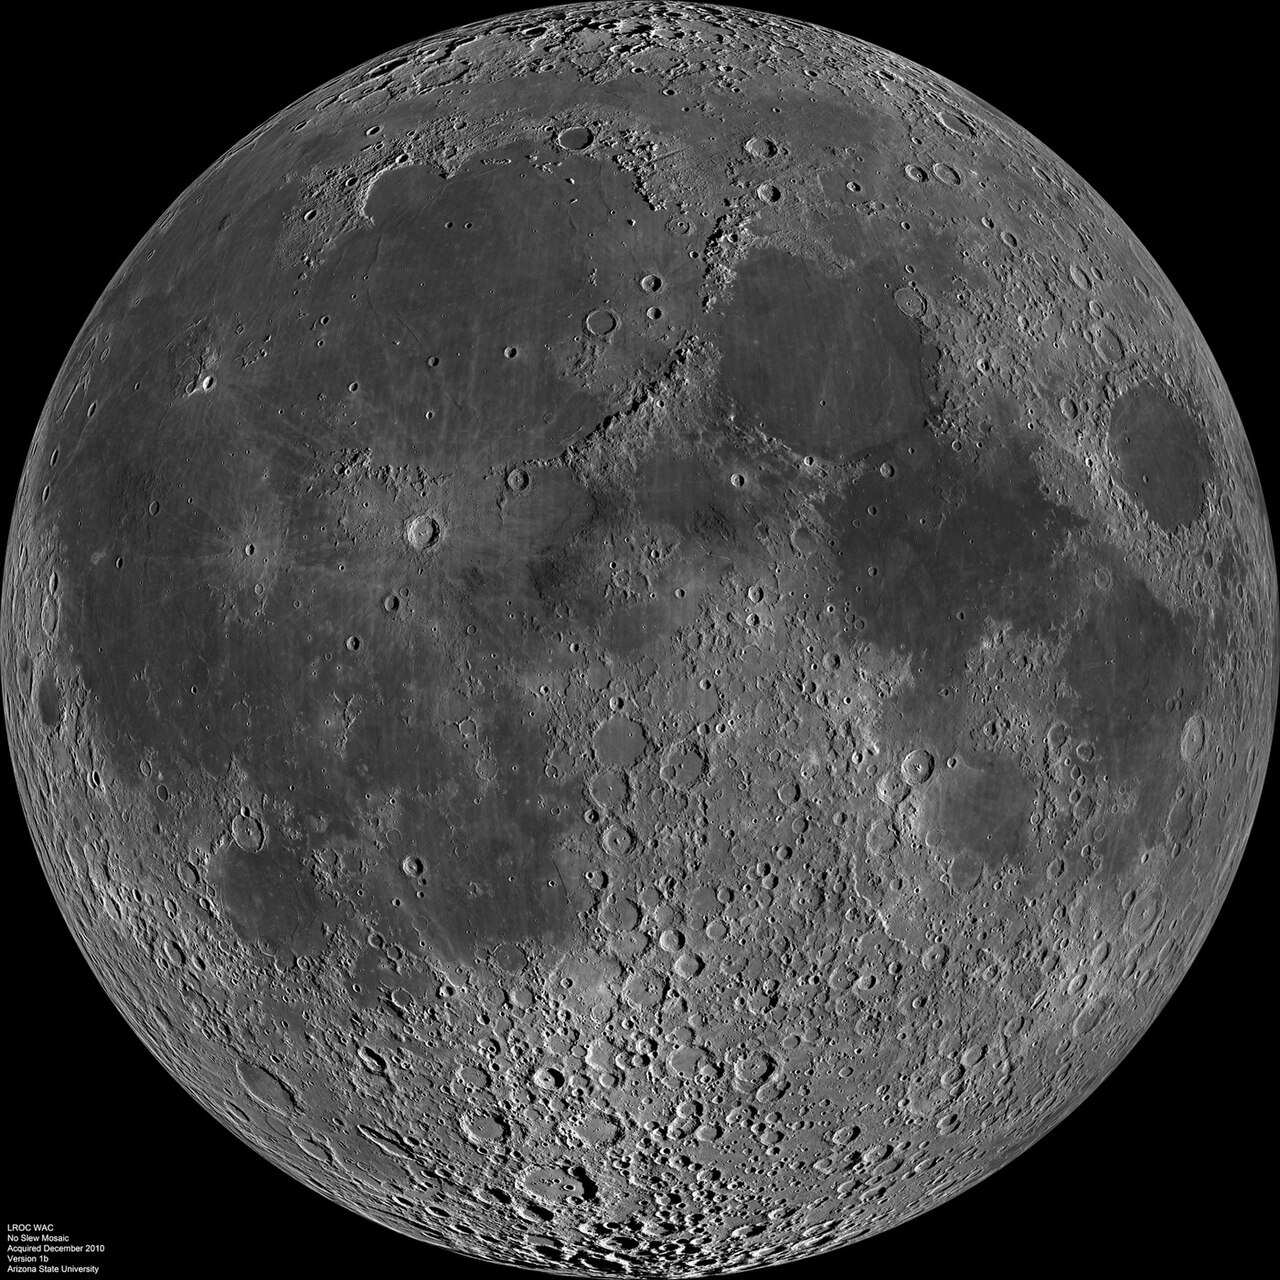
\includegraphics[width=0.40\linewidth]{images/book3/moon-nearside-lro.jpg}

{\small 月球正面（月球勘测轨道飞行器，NASA）：周末问题中望远镜的观测目标，在 \qty{384000}{km} 距离上直径为 \qty{3476}{km}。}
\end{omfigure}

\section{问题：为月球设计一台望远镜}

\begin{problem}[{周末问题——在草坪上使用一台 150 毫米折射望远镜：
选择目镜、确定眼睛位置、计算光量，
并求它能分辨的最小陨石坑}]
\label{pb:b1:optical-instruments:1}
\omterm{def:b1:optical-instruments:microscope}{物镜}为会聚\omterm{def:b1:mirrors-thin-lenses:lens}{透镜} $L_1$，\omterm{def:b1:mirrors-thin-lenses:lens}{焦距}
$f_1' = \qty{1200}{mm}$，直径 $D = \qty{150}{mm}$；可用\omterm{def:b1:optical-instruments:microscope}{目镜}
$L_2$ 的\omterm{def:b1:mirrors-thin-lenses:lens}{焦距}分别为 \qty{25}{mm} 和 \qty{6}{mm}。
月球距离 \qty{3.84e5}{km}，对\omterm{def:b1:optical-instruments:eye}{眼睛}的张角为 $0.52^\circ$；\omterm{def:b1:optical-instruments:eye}{眼睛}的
夜间瞳孔为 \qty{7}{mm}，其分辨率 $\epsilon = \qty{3.0e-4}{rad}$；
$\lambda = \qty{550}{nm}$。

\medskip
\noindent\textbf{第一部分——无焦装置。}
\begin{enumerate}
  \item 星光无需\omterm{def:b1:optical-instruments:eye}{调节}即可看到，\omterm{def:b1:optical-instruments:microscope}{目镜}应放在何处？
        分别给出两个\omterm{def:b1:optical-instruments:microscope}{目镜}各自的
        \omterm{def:b1:optical-instruments:microscope}{物镜}与\omterm{def:b1:optical-instruments:microscope}{目镜}间距。
  \item 对每个\omterm{def:b1:mirrors-thin-lenses:lens}{透镜}依次应用\omterm{thm:b1:mirrors-thin-lenses:lensconj}{笛卡儿关系}，
        验证轴上无穷远处的点成像于无穷远处。
  \item 证明：与轴成 $\alpha$ 角的星光束
        以平行光束射出，出射角为 $\alpha' = -(f_1'/f_2')\alpha$。
  \item 计算两个\omterm{def:b1:optical-instruments:microscope}{目镜}各自的 $G$，以及
        月球经每个\omterm{def:b1:optical-instruments:microscope}{目镜}所见的视直径。
  \item 像是倒立的。此处为何可以接受，
        地面观察镜又会增加什么？
  \item 月球的实中间像位于何处，
        其直径是多少？（它可以在该处拍照。）
\end{enumerate}

\medskip
\noindent\textbf{第二部分——\omterm{def:b1:optical-instruments:eye}{眼睛}的位置。}
\begin{enumerate}[resume]
  \item 证明\omterm{def:b1:optical-instruments:microscope}{目镜}对\omterm{def:b1:optical-instruments:microscope}{物镜}边缘形成一个\omterm{def:b1:mirrors-thin-lenses:image}{实像}，
        位于其后 $\overline{O_2P'} = f_2'(f_1' + f_2')/f_1'$ 处，
        直径为 $D/\abs G$（即出射光瞳）。
  \item 计算每个\omterm{def:b1:optical-instruments:microscope}{目镜}对应的
        出射光瞳的位置与直径。
  \item 为何眼瞳必须置于出射光瞳处？
        若将其置于更靠后的位置，视场会如何变化？
  \item 要使星光被充分利用，出射光瞳不得超过
        眼瞳，由此推出夜间使用时该望远镜的最小有效
        放大率。
\end{enumerate}

\medskip
\noindent\textbf{第三部分——分辨率。}
\begin{enumerate}[resume]
  \item 计算衍射极限 $\theta_{\min} = 1.22\lambda/D$，
        分别以弧度和角秒表示。
  \item 此角度对应月球上最小的陨石坑有多大？
        肉眼又如何？
  \item 定义并计算分辨放大率 $G_r =
        \epsilon/\theta_{\min}$。哪个\omterm{def:b1:optical-instruments:microscope}{目镜}与之最接近？
  \item 使用 \qty{6}{mm} \omterm{def:b1:optical-instruments:microscope}{目镜}时，像比使用 \qty{25}{mm} \omterm{def:b1:optical-instruments:microscope}{目镜}时更模糊、
        更暗。请解释这两种效应。
  \item 大气湍流将星像模糊至约 $1''$。对于哪些\omterm{def:b1:optical-instruments:microscope}{物镜}直径，
        从地面观测时瑞利极限不再构成限制？
        更大的 $D$ 又能带来什么？
\end{enumerate}

\medskip
\noindent\textbf{第四部分——光。}
\begin{enumerate}[resume]
  \item \omterm{def:b1:optical-instruments:microscope}{物镜}比夜间瞳孔多收集了
        多少倍的光？
  \item 将其换算为星等（$\Delta m = 2.5\log_{10}$ 的比值）；
        若\omterm{def:b1:optical-instruments:eye}{眼睛}能看到星等 $6$，则
        望远镜能达到的星等是多少？
  \item 满月在地面的辐照度约为
        \qty{2e-3}{W/m^2}。进入\omterm{def:b1:optical-instruments:microscope}{物镜}的功率是多少？
        它在\omterm{def:b1:optical-instruments:eye}{视网膜}上如何分布，与肉眼观察相比有何不同（
        以单位立体角功率为依据的论证：
        比较两个\omterm{def:b1:optical-instruments:microscope}{目镜}下的表面亮度）？
  \item 为何望远镜不会使月球表面每单位面积比
        肉眼更亮，而它却能使恒星
        变亮？
\end{enumerate}

\medskip
\noindent\textbf{第五部分——视场。}
\omterm{def:b1:optical-instruments:microscope}{目镜}的焦平面上装有一个圆形视场光阑，
直径为 \qty{20}{mm}（\qty{25}{mm} \omterm{def:b1:optical-instruments:microscope}{目镜}）或 \qty{5}{mm}
（\qty{6}{mm} \omterm{def:b1:optical-instruments:microscope}{目镜}）。
\begin{enumerate}[resume]
  \item 证明：真实视场为 $2\arctan(\phi/2f_1')
        \approx \phi/f_1'$，其中光阑直径为 $\phi$。
  \item 计算两个\omterm{def:b1:optical-instruments:microscope}{目镜}的真实视场，并说明
        整个月球能否落入视野之中。
  \item 计算两个\omterm{def:b1:optical-instruments:microscope}{目镜}各自的表观视场（即\omterm{def:b1:optical-instruments:eye}{眼睛}透过\omterm{def:b1:optical-instruments:microscope}{目镜}
        看到光阑所张的角）。
  \item 地球每秒钟自转 $15''$。在不跟踪的情况下，
        月球穿过各\omterm{def:b1:optical-instruments:microscope}{目镜}视场需要多长时间？
  \item 总结此设计：哪个\omterm{def:b1:optical-instruments:microscope}{目镜}用于观察整个月球，哪个用于观察
        陨石坑，以及该仪器能分辨的最小陨石坑尺寸——
        即它唯一的一个数值。
  \item 将同一\omterm{def:b1:optical-instruments:microscope}{物镜}换成\omterm{def:b1:mirrors-thin-lenses:lens}{焦距}相同的 \qty{150}{mm} \omterm{def:b1:mirrors-thin-lenses:mirror}{凹面镜}，
        上述结果中哪些会改变？
\end{enumerate}
\end{problem}
